\chapter{Class F Detailed Description }

The class F amplifier is able to achieve high efficiency by using the harmonics generated during amplification to ideally produce a square wave for the drain voltage and a half sinusoid for the drain current that don't overlap. This allows for ZVS and ZVDS conditions to occur so ideally no power is consumed during amplification. The class F amplifier theoretically capable of 100\% drain efficiency but in practice only a finite amount of harmonics can be matched and the drain capacitance will eventually short the harmonics, the actual typical efficiency is around 80\% to 90\%. Through Fourier series analysis it can be shown that by loading the drain so that odd voltage harmonics see an open circuit and even current harmonics see a short circuit, the ideal current and voltage waveforms conditions will arise \cite{Gao2006}. The class F amplifier also has a counterpart, the class F$^{-1}$ in which the current and voltage waveforms are opposite so that ideally the voltage waveform is a square wave and the current is a half sinusoid which will be discussed later in this chapter \cite{Moon2012}.

\section{Fourier Analysis}

Power amplifiers typically operate in the large signal mode which includes the non-linear region of a transistor. This results in harmonic and intermodulation distortion but can also be used to increase the efficiency of the amplifier. The source of the harmonics in power amplifiers is attributed to the knee voltage of the device. The knee voltage essentially clips the peak of the drain current and due to the relatively large discontinuity harmonics are generated \cite{Colantonio1998}. The current source amplifier theory doesn't predict the effect of the knee voltage in analysis but as seen in Figure \ref{fig:knee_harmonics} even in the class B amplifier the knee voltage will cause a discontinuity. No rigorous analysis that shows the relation of the knee voltage to the harmonic generation has been done but measurements have verified the presence of harmonics.

\begin{figure}
  \centering
  % Requires \usepackage{graphicx}
  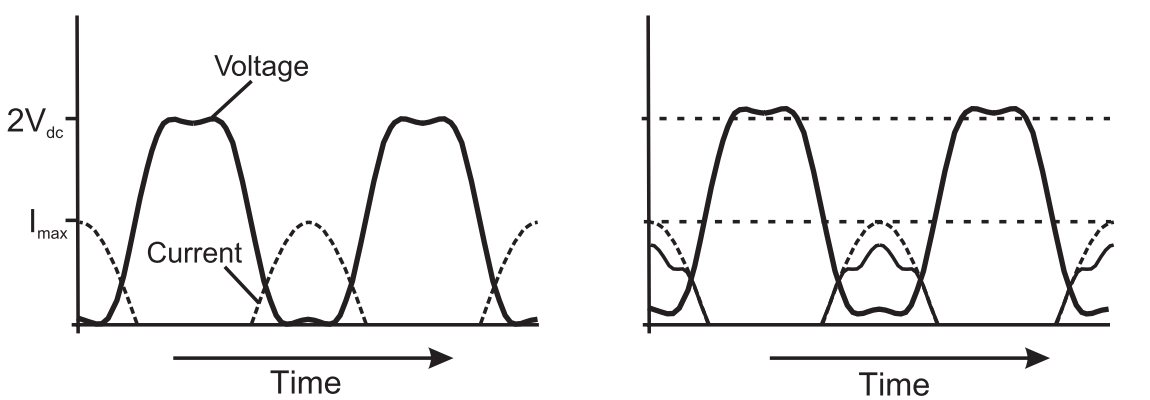
\includegraphics[width=6in,height=6in,keepaspectratio]{figures/detail/knee_harmonics}\\
  \caption{Transient Waveforms of Class B Amplifier With and Without Knee Voltage \cite{C.Cripps2006}}
  \label{fig:knee_harmonics}
\end{figure}

For simplified a discussion it is assumed the DC bias of the amplifier is set so the conduction angle is $\pi$, like the other switching amplifiers, so the drain current waveform can be modeled as a half sinusoid. It will be shown later that in practice the conduction angle should be close to $\pi$ but not exactly $\pi$ but to explain the ideal case the conduction angle should be $\pi$. The drain current and voltage waveforms can be modeled as a Fourier series with odd components for the voltage and even for the current as seen in Equations \ref{eq:current_inf_series} and \ref{eq:voltage_inf_series} \cite{Raab1997}. 

\begin{equation}\label{eq:current_inf_series}
  i_{d}(t) = I_{DD} - I_{f0}sin(\omega t) - I_{2f0}sin(2\omega t) - I_{4f0}sin(4\omega t) + \ldots
\end{equation}

\begin{equation}\label{eq:voltage_inf_series}
  v_{d}(t) = V_{DD} + V_{f0}sin(\omega t) + V_{3f0}sin(3\omega t) + V_{5f0}sin(5\omega t) + \ldots
\end{equation}

%Insert picture of ideal class F waveforms and related them to the picture
%Insert references to the parameter equations

From Equations \ref{eq:current_inf_series} and \ref{eq:voltage_inf_series}, four new parameters: $\gamma_v, \gamma_i, \delta_v \ and \ \delta_i$ relate the fundamental and peak amplitude to the DC component for the drain and voltage. These parameters can be used to define the ideal load at the fundamental frequency, RF output power at the fundamental frequency, DC input power, and the drain efficiency seen in Table \ref{table:class_f_param} from \cite{Raab1997}. The key take away from the all equations this is that the drain efficiency can be described as a function of $\gamma_v$ and $\gamma_i$, which are the voltage and current ratios at the fundamental frequency to the DC amplitude.

\begin{table}
    \centering

    \label{table:class_f_param}
    \caption{Various Parameters of Maximally Flat Waveforms for Class F Amplifier }

    \begin{tabular}{|l|l|}
      \hline
      % after \\: \hline or \cline{col1-col2} \cline{col3-col4} ...
      {Equation} & {Description} \\ \hline
      { $\gamma_v = \frac{V_{f0}}{V_{DD}} $ } & {Voltage Ratio of Fundamental Amplitude to DC Amplitude} \\ \hline

      { $\gamma_i = \frac{I_{f0}}{I_{DD}}$ } & {Current Ratio of Fundamental Amplitude to DC Amplitude} \\ \hline

      { $\delta_v = \frac{v_{max}}{V_{DD}}$} & {Ratio of Maximum Drain Voltage to DC Amplitude} \\ \hline

      { $\delta_i = \frac{i_{max}}{I_{DD}}$} & {Ratio of Maximum Drain Current to DC Amplitude} \\ \hline

      { $Z = \frac{V_{f0}}{I_{f0}}$}    & {Optimal Impedance at Fundamental for Max Power Transfer} \\ \hline

      { $P_{o,f0} = \frac{V^2_{f0}}{2Z} = \frac{\gamma_v^2 V_{DD}^2}{2Z}$} & {Output Power at Fundamental} \\ \hline

      { $P_i = V_{DD} I_{DD} = \frac{\gamma_v V_{DD}^2}{\gamma_i Z}$}      & {DC Input Power} \\ \hline

      { $\eta = \frac{P_{o,f0}}{P_i} = \frac{\gamma_v \gamma_i}{2}$}       & {Drain Efficiency} \\ \hline
    \end{tabular}
\end{table}

The $\gamma$ and $\delta$ parameters can be extended for all the harmonics and is used to describe what is called maximally flat waveforms. The term maximally flat refers to the ideal scenario were all the odd harmonics of the drain voltage see an open circuit and the even harmonics of the voltage are shorted. And all the even harmonics of the drain current see a short circuit and the odd harmonics are shorted at the drain which results in the square wave for the drain voltage which has a flat top that doesn't overlap with the half sinusoid drain current seen in Figure \ref{fig:classf_wave}. The ideal waveforms allow for the ZVS and for ZVDS condition to occur so zero power would be consumed in the switching operation and all of the DC input power would be used to increase the input power so the PAE would also be 100\%.

%insert figure of ideal class F waveforms

Fourier series analysis can be used to determine the amplitudes of each harmonics in Equation \ref{eq:current_inf_series} and \ref{eq:voltage_inf_series} for a maximally flat waveform. In the ideal case were infinite number of odd voltage harmonics can be properly terminated, the amplitude of the each harmonic is that of a square wave seen in Equation \ref{eq:fs_squarewave}. For the ideal case for terminating all the even current harmonics, the amplitude of each harmonic is equal to that of a half sinusoid in Equation . For the ideal case, $\gamma_v = \frac{4}{\pi}$ and $\gamma_i = \frac{\pi}{2}$ and from Table \ref{table:class_f_param}, $\eta = \frac{\gamma_v \gamma_i}{2} = \frac{ \frac{4}{\pi} \frac{\pi}{2} }{2} = 100\%$. The efficiency is dependent on the input power because of required harmonic level to produce the maximally flat waveforms. As input power is backed off, the harmonic levels and efficiency drops as well and the class F amplifier becomes more like a class A amplifier. The class F amplifier has a counterpart, the class F$^{-1}$ amplifier which swaps the voltage and current waveforms so the ideally the drain current is a square wave and the voltage is a half sinusoid.

\begin{figure}
  \centering
  % Requires \usepackage{graphicx}
  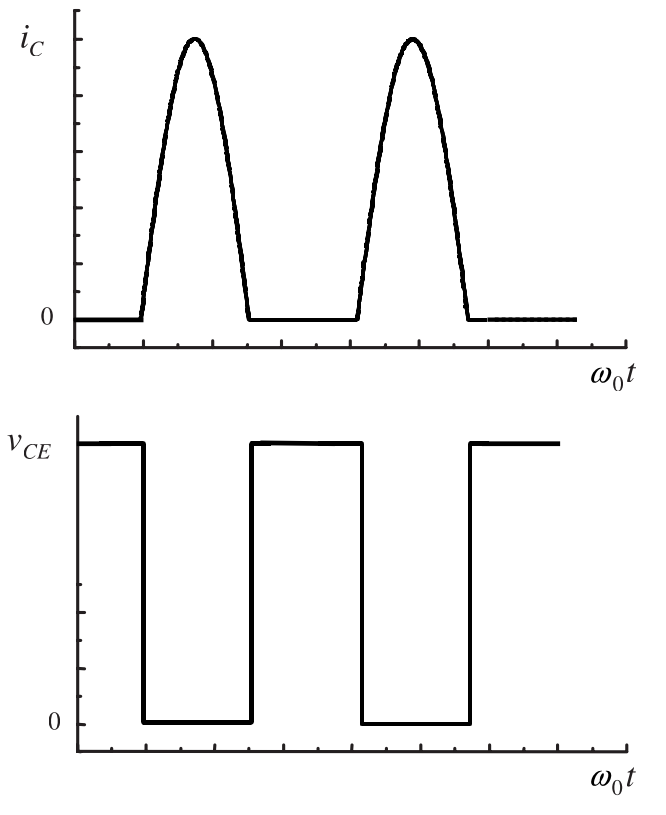
\includegraphics[width=4in,height=4in,keepaspectratio]{figures/detail/classf_wave}\\
  \caption{Ideal Class F Waveforms \cite{Rudiakova2006}}
  \label{fig:classf_wave}
\end{figure}

%Theoretically it has the same properties as the class F amplifier and experimentally it has been show to do things. Flesh this out.

%Now after showing how harmonics increase efficiency talk about about how harmonics are kept at the drain using harmonic matching

In practice, a matching network to terminate infinitely many harmonics is impossible and the output drain capacitance of the transistor will short out higher harmonics. Typically as a compromise between feasability and efficiency, up to the third harmonic is terminated which is called third harmonic peaking. This is more common in class F amplifiers that operate in the couple of gigahertz which can take advantage of the high transition frequency of new technologies like high electron mobility (HEMT) transistors. In the high frequency (HF) and very high frequency (VHF) domain, higher harmonics are present and are typically more efficient than their gigahertz counterparts.

To solve for the harmonic amplitude of each component when only a finite number of harmonics are terminated, the derivatives of Equation \ref{eq:voltage_inf_series} and \ref{eq:current_inf_series} are solved with the condition at $\omega t = \frac{3\pi}{2}$, $v_d=0$ and all higher harmonic amplitudes are set to 0. For example for terminating up to the third harmonic, the second derivative for the voltage, seen in Equation \ref{eq:fs_2nd_derv}, with the conditions applied is $0 = V_{f0} - 9V_{3f0}$, therefore $V_{3f0} = \frac{1}{9} V_{f0}$. Then using Equation \ref{eq:voltage_inf_series} with the same conditions, $V_{f0}=\frac{9}{8}V_{DD}$ and $V_{3f0} = \frac{1}{8}V_{DD}$. The same process applied to the current waveform results in $I_{f0}=\frac{4}{3}I_{DD}$ and $I_{2f0} = \frac{1}{3}I_{DD}$. The drain efficiency for terminating up to the third harmonic can now be calculated, $\eta = \frac{\gamma_v \gamma_i}{2} = \frac{ \frac{9}{8} \frac{4}{3} }{2} = 75\%$. A table of how efficient the class F amplifier for a finite number of harmonic terminations can be seen in Table \ref{table:harmonic_eff}. Going back to the current source amplifiers, the class A amplifier only controls the first harmonic of the current and voltage and from Table \ref{table:harmonic_eff} it's only 50\%. The class B amplifier controls only the first voltage harmonic and ideally all of the current harmonics and is ideally 78.5\% efficient. %insert table of harmonic matching

%Talk about max power output compared to class A amplifiers! Can use the gamma and delta equations
% Or talk about power back off and how it reduces to a class A amplifier

%Talk about inverse class F amplifier

\begin{table}
    \caption{Maximum Efficiency of Class F Amplifier}
    \label{table:harmonic_eff}
        \begin{center}
            \begin{tabular}{|l|l|l|l|l|}
              \hline
              % after \\: \hline or \cline{col1-col2} \cline{col3-col4} ...
              Harmonics    & $n = 1$ & $n =  3$ & $n = 5$ & $n = \infty$ \\ \hline
              $m = 1 $     & 50.0\% & 57.7\% & 60.3\% & 63.7\% \\ \hline
              $m = 2 $     & 70.7\% & 81.7\% & 85.3\% & 90.0\% \\ \hline
              $m = 4 $     & 75.0\% & 86.6\% & 90.5\% & 95.5\% \\ \hline
              $m = \infty $& 78.5\% & 90.7\% & 94.8\% & 100\% \\ \hline
            \end{tabular}
            \text{m,n are the maximum order of drain current and voltage harmonics}
        \end{center}
\end{table}

\begin{equation}\label{eq:fs_2nd_derv}
  \frac{d^2 v_d}{d \theta^2} = -V_{f0}sin(\omega t) -9V_{3f0}sin(3\omega t) - 25V_{5f0}sin(5\omega t) + \ldots
\end{equation}

%\begin{equation}\label{eq:fs_4th_derv}
%  \frac{d^4 v_d}{d \theta^4} = V_{f0}sin(\omega t) + 81V_{3f0}sin(3\omega t) + 625V_{5f0}sin(5\omega t) + \ldots
%\end{equation}

\begin{equation}\label{eq:fs_squarewave}
    V_{mf0} = \frac{4}{m\pi}
    \begin{cases}
        0, & \text{if}\ m = even\\
        1, & \text{if}\ m = odd\\
    \end{cases}
\end{equation}

%\begin{equation}\label{eq:fs_halfsinusoid}
%
%\end{equation}

\section{Practical Implementation}

A key factor that is missing from the Fourier analysis of the waveforms is the phase relation between the harmonics, if all of the harmonics are in phase the amplifier will have a much lower efficiency due to destructive interference. This can especially be seen in third harmonic peaking amplifiers seen in Figure \ref{fig:third_harmonic_phase}. The right part of the figure shows the drain voltage if the third harmonic is in phase. This results in triangle wave instead of a square wave which would overlap with the half sinusoidal current. The left part of the figure shows the drain voltage with an out of phase third harmonic which results in the proper square wave shape. Going back to Figure \ref{fig:bias_current_harmonic}, in order for the third harmonic to be out of phase the class F amplifier must be biased between so the conduction angle is between $\pi$ and $2\pi$. Within these conduction angles, the third harmonic is negative relative to the fundamental so it is out of phase. For conduction angles less than $\pi$, the third harmonic will be in phase and will result in a loss of efficiency. In practice, the class F amplifier is biased in the so called "deep AB" region so that it slightly greater than a conduction angle of $\pi$ so the drain current will still resemble a half sinusoid shape and the voltage waveform will be maximally flat.

\begin{figure}
  \centering
  % Requires \usepackage{graphicx}
  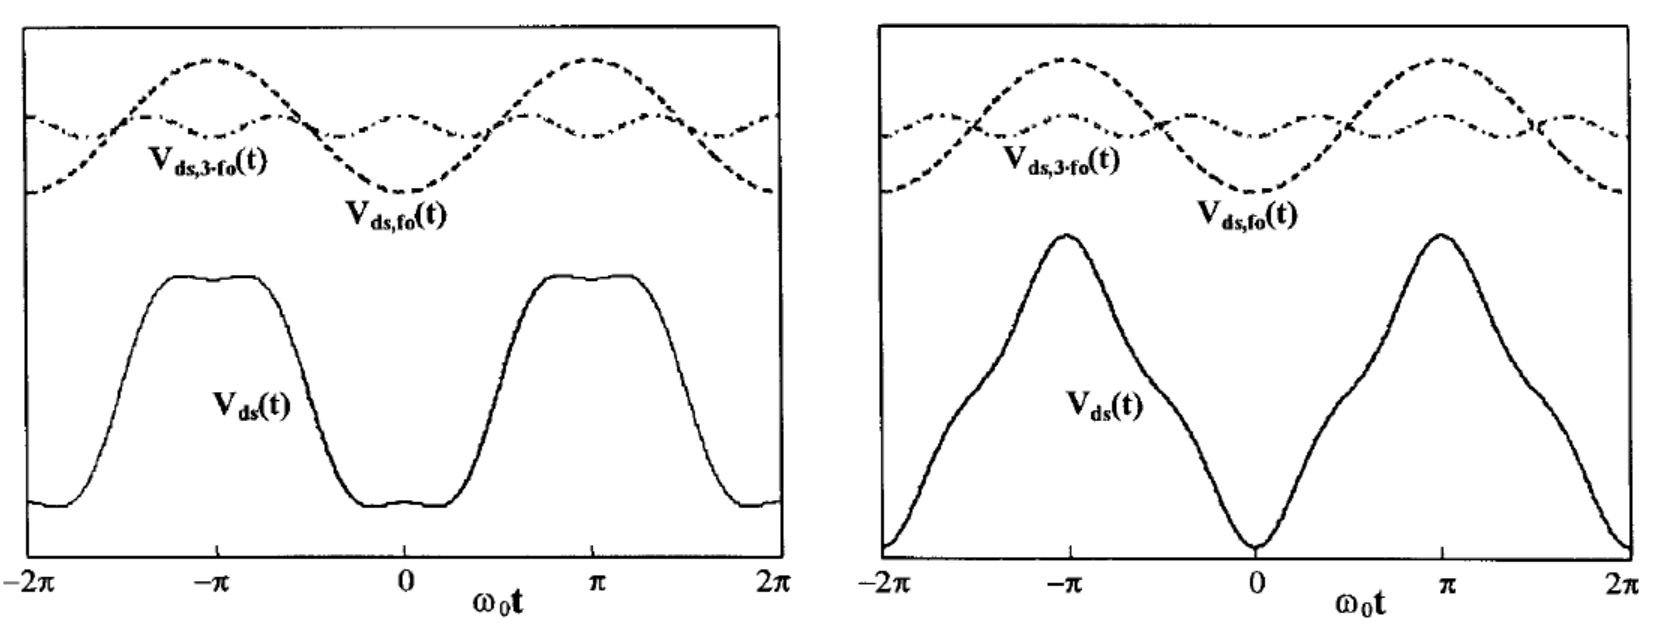
\includegraphics[width=5in,height=5in,keepaspectratio]{figures/detail/third_harmonic_phase}\\
  \caption{Drain Voltage Waveform with In Phase and Out of Phase Third Harmonic \cite{Colantonio1998}}
  \label{fig:third_harmonic_phase}
\end{figure}

The design of a class F amplifier starts with finding a suitable "deep" AB bias with sufficient gain for the application. Then applying a load pull at the fundamental frequency to determine the optimal load impedance, and then a source pull at the fundamental frequency for the optimal source impedance. Load pulling and source pulling are measurements that measure the s-parameters of a device while applying it to a uniformly sampled smith chart on the load and source side while the source and load impedance respectively is held constant. Simulated load pulls require accurate device models to be of any use and to take real world load pull measurements are time intensive without automated test equipment. After determining the optimal load and source impedances, a harmonic phase load pull is done which is similar to a load pull, but applied to a harmonic frequency and the smith chart is sampled uniformly in phase at a constant gamma value. For the class F amplifier to keep the drain current and voltage harmonics at the drain, the odd harmonics have to see a open and the even harmonics a short.%DOUBLE CHECK THIS STATEMENT.
The harmonic phase load pulls are done at a reflection coefficient value of 1 and swept to measure the transistor efficiency if the harmonics are terminated properly. This process is usually iterated until a proper bias is found that allows for sufficient gain and the load pulling results in the desired efficiency.

\section{Matching Networks}

The matching network for a class F amplifier can be down with passive components, some closed form methods use the output drain capacitance and impedance as parameters to come up with matching networks but this has only been shown to work in sub 1 GHz band \cite{Grebennikov2000}. Multiple papers show that the output capacitance is non-linear at higher frequencies and some work has explored methods to make compensate for the non-linearity using varactors \cite{Kye-Ik1997}. The most common methods rely on resonant transmission line matching networks which are intuitive to a certain degree. The simplest transmission line matching network for the class F amplifier uses a quarter wavelength line at the drain to a tuned load as seen in Figure \ref{fig:quarter_wave_match}. The tuned load is such that at odd harmonics it appears as a short and even harmonics an open, so when reflected back at the drain the odd harmonics see an open and even harmonics a short \cite{Gao2006}. In practice with this type of matching network, the impedances of the various sections are parameterized and are left to be found by an optimizer using simulation software. It's also been experimentally determined that a harmonic matching network at the input of the transistor increases the efficiency over just having a matching network at the output \cite{Colantonio2001}.

\begin{figure}
  \centering
  % Requires \usepackage{graphicx}
  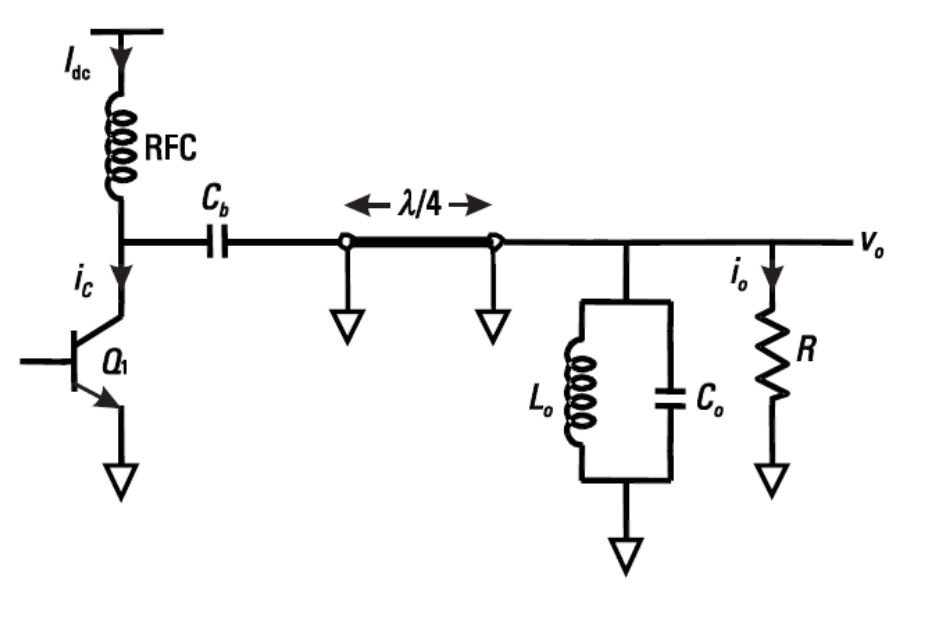
\includegraphics[width=4in,height=4in,keepaspectratio]{figures/detail/quarter_wave_match}\\
  \caption{Quarter Wavelength Matching Network for Class F Amplifiers}
  \label{fig:quarter_wave_match}
\end{figure}


%When using the class F amplifier in the real world the biggest difference from theory to practice is the number of harmonics that can be matched. The shunt drain capacitance on the transistor will reduce the amplitude of a higher harmonics and designing harmonic matching networks for more than a few harmonics becomes cumbersome. In most cases the tradeoff for efficiency and feasibility lies at matching up to the third harmonic, this technique is called third harmonic peaking.

%There are some closed form solutions using lumped elements but not the best. Many of the published solutions have an intuitive wavelength matching, but the impedances of the transmission lines are arrived by doing a combination of load pull and source pull of the transistor at each harmonic and optimizing the impedances for gain or efficiency. Class F amplifier is a narrow band amplifier due to the matching requirements

%Also experimentally that having harmonic matching networks at the input is also needed to increase efficiency 